\chapter{腹部钝伤}

\section{检查方法}

\subsection{检查前准备}

对于危急患者可直接进行扫描。对尚能配合的患者且在病情允许的情况下,于扫描前30~45分钟口服或鼻饲管给予1.5%~2%泛影葡胺500ml,上床时再服250ml。对于不能控制活动的病人,为避免运动伪影,可服用一定量的镇静剂,或采用动态快速扫描。

\subsection{扫描方法}

以层厚和层间隔10mm扫描,上腹部以动态扫描或螺旋扫描为佳。中下腹部多采用非动态扫描,层间距可适当加大。增强扫描以2~3ml/s流率注入造影剂100ml,小儿剂量为2~3ml/kg体重,做动态或螺旋扫描。

多数学者主张以增强扫描来发现肝、脾损伤,而避免做平扫。但国内有学者亦主张当要了解肝、脾及肾血供时,才做增强检查。

\section{腹腔积血}

腹腔内积血是腹部顿伤的常见征象。腹腔内任何液体包括血液首先分布于附近间隙,然后流到更低的间隙如肝肾间隙、左右膈下、左右结肠旁沟或盆腔的Douglas窝。

\subsection{出血量的判断}

①如果腹腔内积血存在于1个间隙,约有100~200ml,称为少量积血;②如包括两个间隙,约有250~500ml,为中量积血;③大量积血指积血量>500ml,包括两个以上间隙,可在盆腔内看到积血。还有学者报道1000ml以上腹血者,CT表现其前后径均>1.5cm。但CT对腹血量的估计有一定限度。

\subsection{CT表现}

1.CT值的变化:①急性腹腔积血的CT值平均约45Hu;于20小时内的血块,CT值近于60Hu;②超过48小时,由于蛋白质的破坏和吸收,其CT值降低,但仍>30Hu;③血肿的CT值偏高。

2.腹腔积血与脑出血不同,颅内新鲜血肿为高密度,而腹腔积血多呈低密度(图\ref{fig20-1})。原因如下:①腹部窗宽为200~500Hu,比常规颅脑的窗宽(80~100Hu)要宽的多,由于腹腔的灰度等级宽(每个灰阶内包含的CT值范围大),从而使密度相近的物质减低了对比;②血块的CT值为50Hu左右,而脑的CT值多小于40Hu,故脑内新鲜血肿呈高密度;肝、脾的CT值为50~60Hu,故腹腔积血常呈相对低密度;③腹腔内的血块由于受呼吸运动和附近肠蠕动的影响而迅速溶解,其CT值降低,2~3周左右常达到水样密度,而在脑内和肝内的血块可保持相对的长期稳定。

3.“哨兵血块”征:几乎所有腹部钝伤所致的腹腔积血,其CT值>30Hu,高于一般腹水。而局部血肿或血凝块的CT值更高(>60Hu),且提示邻近脏器损伤的存在,故称为“哨兵血块”征(图\ref{fig20-1})。

\begin{figure}[!htbp]
 \centering
 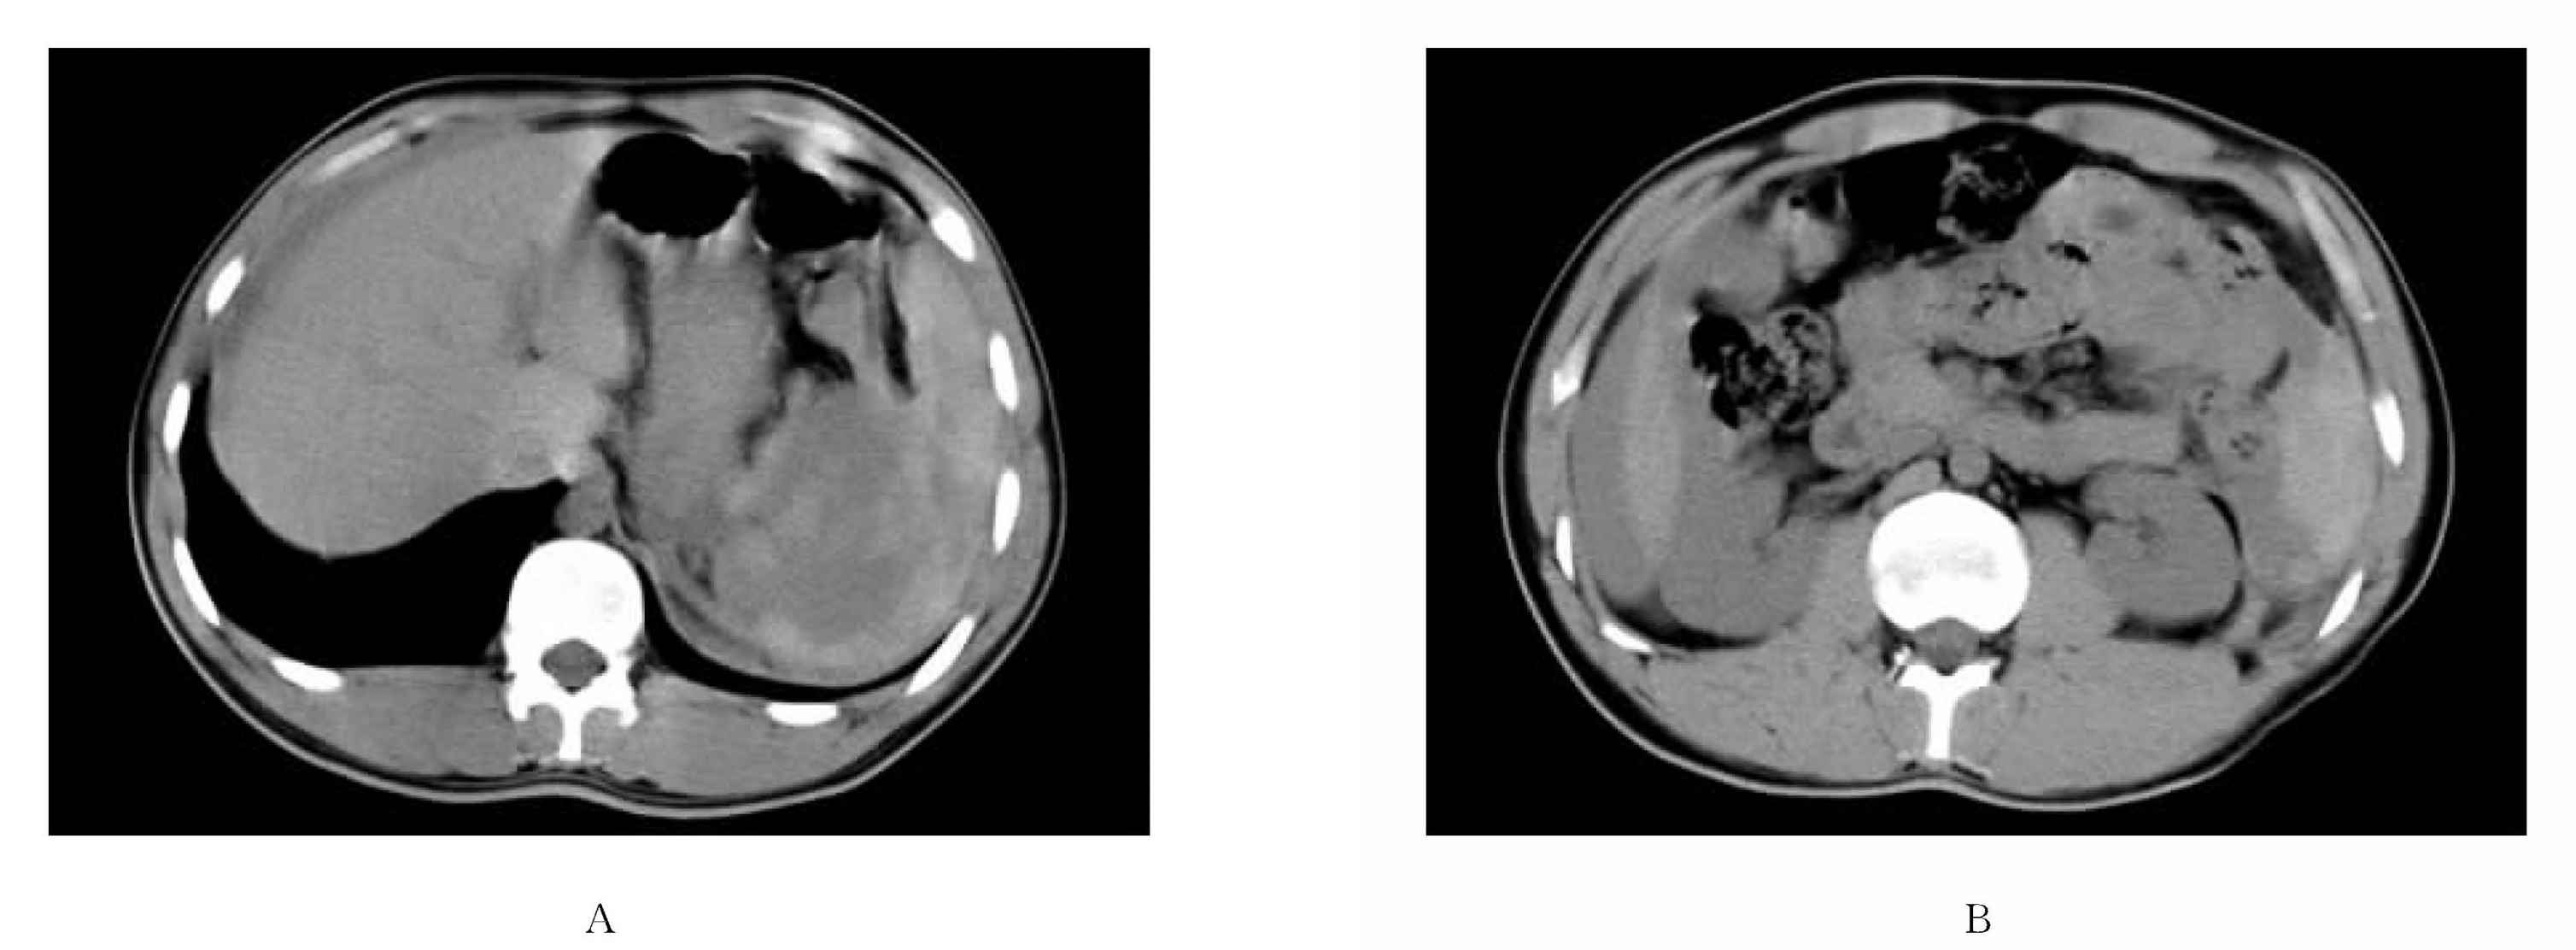
\includegraphics[width=.7\textwidth,height=\textheight,keepaspectratio]{./images/Image00389.jpg}
 \captionsetup{justification=centering}
 \caption{腹腔积血\\{\small A、B为同一患者,肝周可见低密度积血;脾挫裂伤所致,脾内、脾周均有高密度出血灶}}
 \label{fig20-1}
  \end{figure} 

4.腹腔积血对邻近肝、脾无受压表现,有助于与肝、脾包膜下血肿相鉴别。

虽然游离积血呈相对低密度,但由于在损伤后48h内其CT值常>30Hu,仍然高于肝硬化腹水、肾性腹水及大多数渗出性腹水(恶性或炎性的),故游离积血与上述腹水是可以鉴别的。此外,创伤病人的腹腔内积液并不总是血液,少量出血还可能被稀释;创伤病人的腹水、尿液、胆汁或肠内溶液的CT值往往是0~10Hu。

\section{实质性脏器损伤}

\subsection{脾钝伤}

脾损伤是最常见的腹部钝性伤,约占腹部脏器钝伤的40%。

\textbf{【病理】}
可分为以下几类:①脾挫伤;②包膜下血肿:包膜下实质损伤而局部脾包膜完整;③脾实质内损伤而无脾破裂:此时多在脾髓内形成大小不等、形状不规则的血肿;④脾破裂:此时脾实质与包膜均有破裂,除脾内有出血外,脾周围及腹腔内均有积血。也有学者将其分为3种类型,即完全性破裂、中心性破裂、包膜下破裂。

迟发性脾破裂是指伤后2天以上潜伏期,继而突然发生脾脏出血,并出现相应内出血临床表现者,占外伤性脾破裂的5%~15%。

\textbf{【临床表现】}
一般有脾外伤史,但当脾脏本身有病变时,即使无明确的外伤史,也可发生脾脏破裂。脾外伤后可出现左腹部疼痛、脾大和压痛,以及腹膜刺激征。当脾完全破裂时,患者的血红蛋白急速下降,并有休克等严重症状。

\textbf{【CT表现】}

\subsubsection{常见表现}

1.脾包膜下血肿:表现为局限性、新月形或半月形,伴有相应实质受压变平或呈锯齿状,可呈高密度、等密度和低密度。增强扫描有助于血肿的显示。

2.脾实质内血肿:新鲜血肿呈圆形或椭圆形的高密度,随时间推移而呈等密度或低密度区。增强扫描均呈低密度。如脾包膜破裂则形成腹腔积血。

3.脾撕裂:①单一性撕裂:增强扫描见脾实质内线样低密度区。但急性期边缘不清,治愈后呈边缘清楚的裂隙。②多发性撕裂:呈多发性低密度或多发性高密度出血灶,增强扫描呈粉碎脾表现,通常累及脾包膜并伴腹腔积血(图\ref{fig20-2})。③脾脏不强化的楔形低密度区,提示脾脏段的动脉栓塞。

\begin{figure}[!htbp]
 \centering
 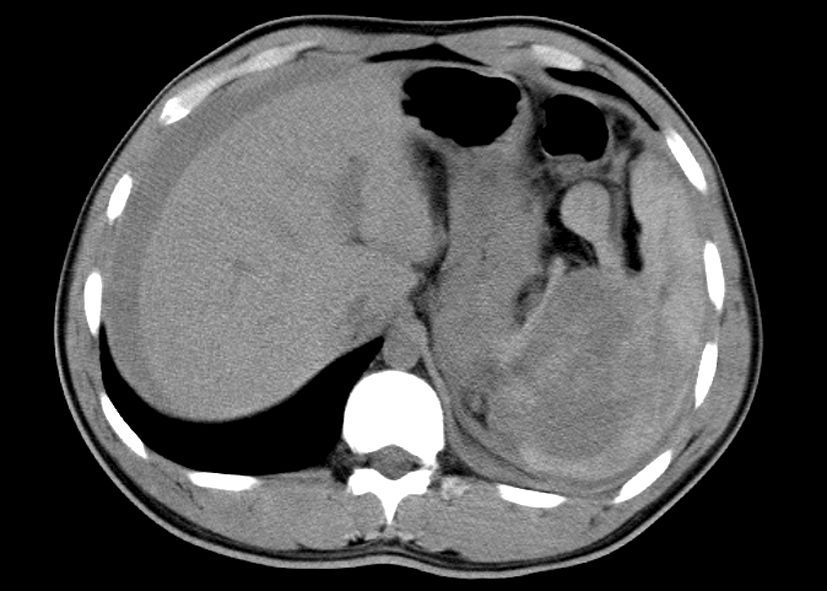
\includegraphics[width=.7\textwidth,height=\textheight,keepaspectratio]{./images/Image00390.jpg}
 \captionsetup{justification=centering}
 \caption{脾撕裂伤\\{\small 脾内可见多发不规则出血灶,脾周亦有高密度出血灶}}
 \label{fig20-2}
  \end{figure} 

此外,脾脏包膜破裂造成腹腔积血占脾损伤的98%,脾周血肿也是脾损伤的常见伴发征象。故当有腹腔积血和脾周血肿时,应仔细寻找有无脾损伤存在,但脾损伤偶尔可仅表现为密度不均匀而看不到撕裂。还应注意排除脾分叶、先天性切迹、肋骨所致伪影等形成的假象。

\subsubsection{迟发性血肿}

无论在实质内还是包膜下,其CT均呈低或略低密度,与新鲜血肿呈高密度不同,可能与出血时间及出血速度有关。迟发破裂常伴有渗出、水肿,加之血肿内血红蛋白随时间而降解,故呈相对低密度。增强扫描有助于血肿的显示。还有学者认为,脾实质细微不均和左肾前筋膜增厚可能是迟发性脾破裂最初的惟一征象。

\textbf{【CT分级】}
其CT分级方法很多,报道不一。国外学者Moore等将其分为5级:Ⅰ级,脾包膜下血肿小于其表面积的10%或撕裂深度<1cm;Ⅱ级,脾包膜下血肿为其表面积的10%~15%,脾实质血肿直径<2cm或撕裂深度1~3cm;Ⅲ级,脾包膜下血肿大于其表面积的50%,脾实质血肿直径>2cm或撕裂深度>3cm;Ⅳ级,脾门损伤,25%以上血供阻断;Ⅴ级,脾脏完全破裂或撕裂,50%~100%的血供阻断。

但CT常常低估了脾损伤的实际程度。一般认为Ⅰ级可以在严密监护下采用非手术治疗,Ⅱ、Ⅲ级主要作修补术,Ⅳ、Ⅴ级宜行脾切除术。

\subsection{肝钝伤}

肝钝伤占腹部脏器钝伤的20%。

\textbf{【病理】}
可分为以下几类:①撕裂伤;②包膜下血肿;③肝实质挫伤;④肝静脉损伤;⑤肝动脉损伤;⑥肝脏胆系的破裂。钝性损伤通常产生肝实质的撕裂伤;肝包膜下血肿通常由于穿透性创伤所致。

\textbf{【临床表现】}
有右侧胸、腹部外伤史。主诉右上腹疼痛,有时向右肩放射。严重时可出现失血性休克,体检多有腹膜刺激征。

\textbf{【CT表现】}

1.肝包膜下血肿:①表现为局限性等密度或低密度区,相应肝实质受压变平。②血肿密度随时间推移而减低,多在6~8周吸收消失。

2.肝实质内血肿:常呈圆形、卵圆形或不规则状密度增高或减低区,边缘多较模糊(图\ref{fig20-3}A、B)。血肿吸收较包膜下血肿慢。在吸收过程中血肿周围出现低密度带环绕,增强扫描时此带可强化。

3.肝撕裂:多位于肝右叶的后段,因这部分肝与肋骨和脊柱相邻;肝左叶的损伤往往是垂直方向上的,是由于自左叶向脊柱从前向后的压力所致。撕裂可以是单一或多发性的,呈单一或多发的线状低密度,边缘模糊(图\ref{fig20-3}C)。1周左右撕裂的边缘可变的清晰,但2~3周后撕裂间隙变窄、边缘可又变模糊。增强扫描可以反映肝块的血供情况,不强化的肝块表示其动脉栓塞或断裂。

4.肝动、静脉的损伤:若撕裂累及主要的肝血管结构如大的肝静脉、门静脉等,可显示邻近血管撕裂处有活动性出血的征象。

5.门静脉轨迹征:即门静脉周围的低密度带,有可能是肝外伤的CT征象,并可能是惟一征象(图\ref{fig20-3}D)。此征被认为是门静脉周围出血或门静脉淋巴回流受阻所致。

\begin{figure}[!htbp]
 \centering
 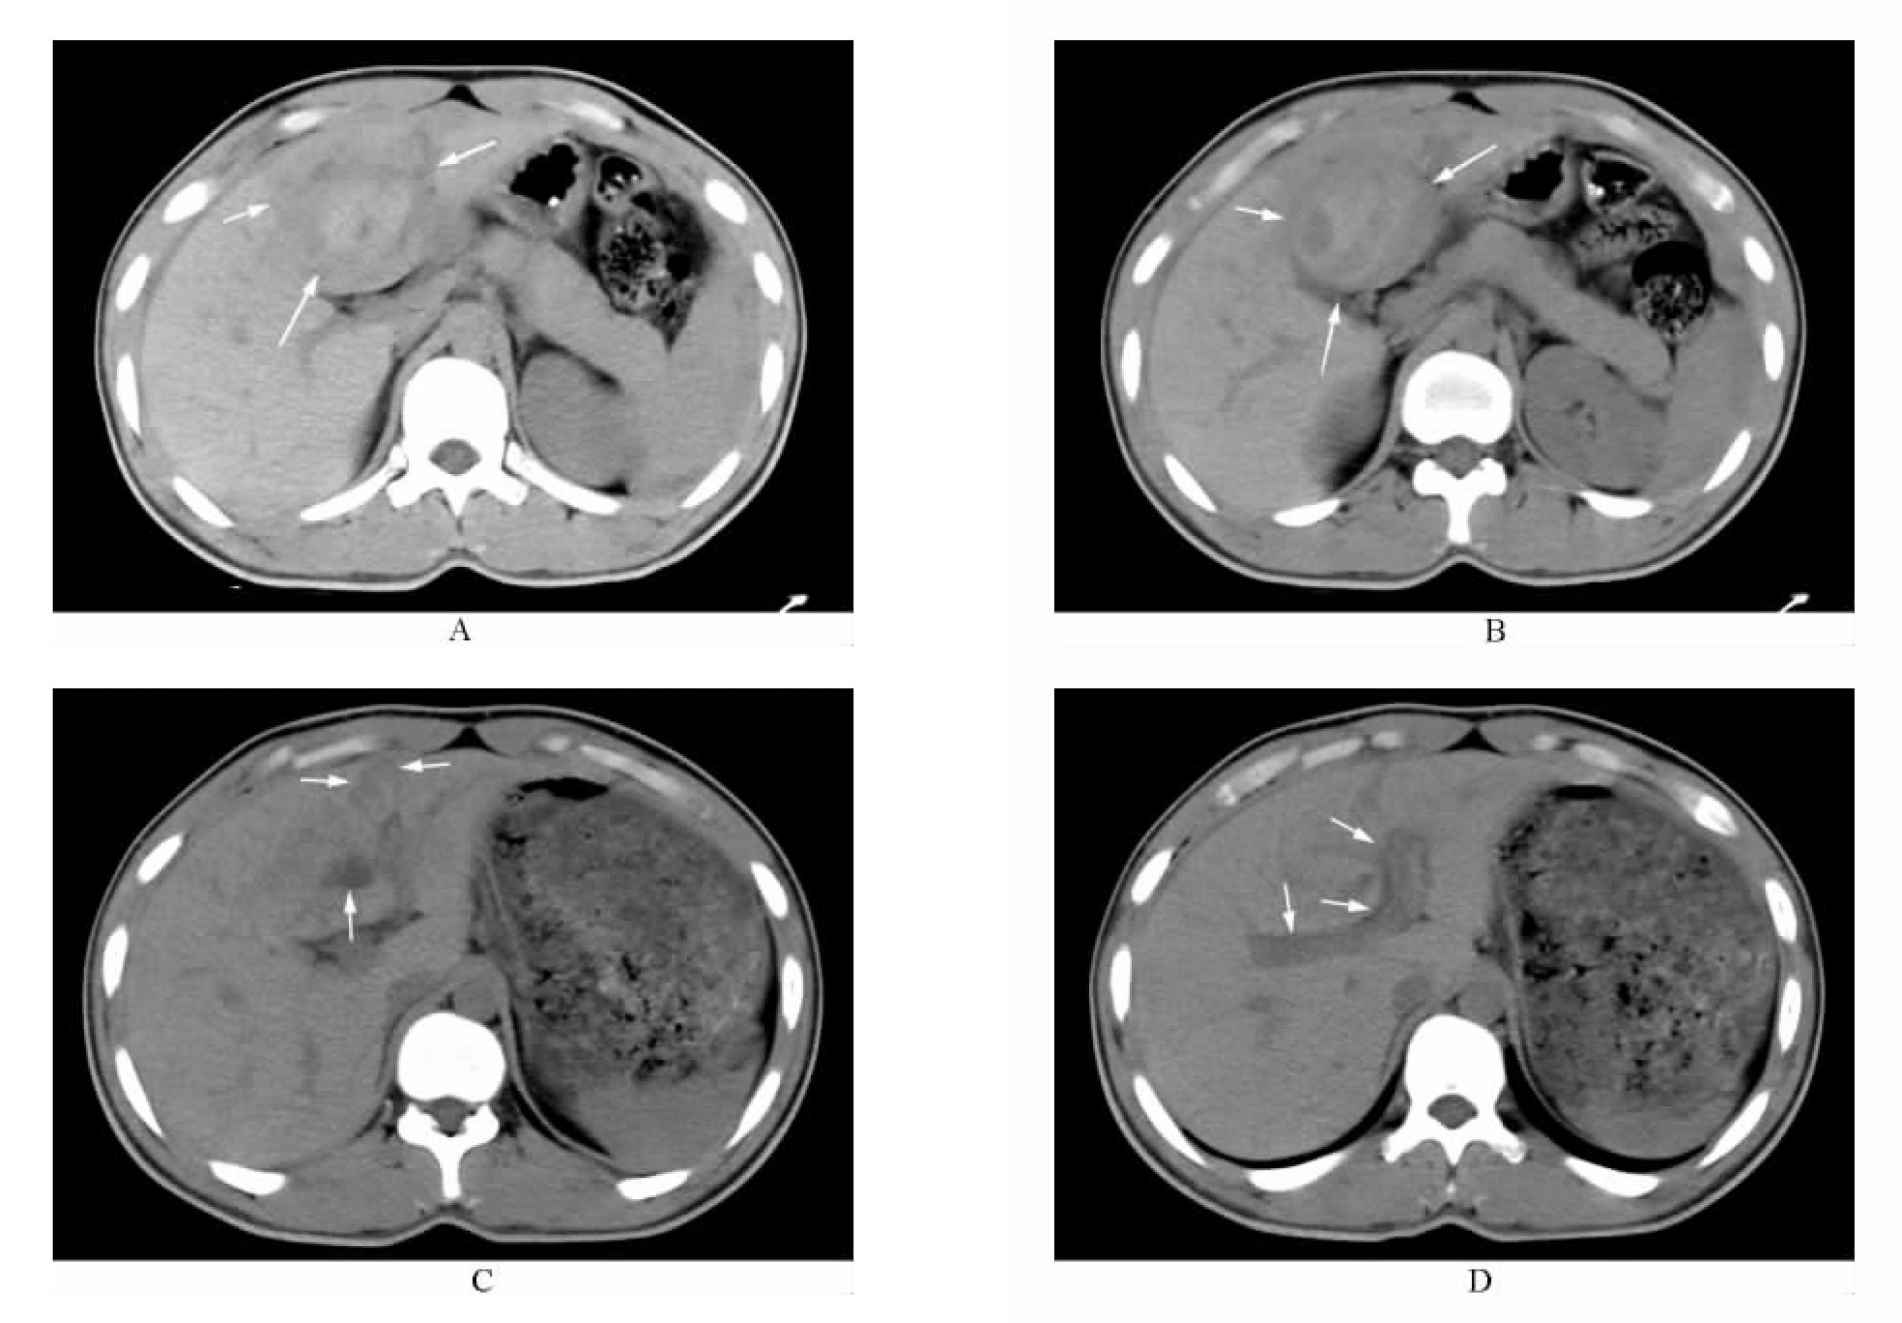
\includegraphics[width=.7\textwidth,height=\textheight,keepaspectratio]{./images/Image00391.jpg}
 \captionsetup{justification=centering}
 \caption{肝钝伤\\{\small A~D为同一患者。A、B为外伤后7天,表现为肝实质内血肿,左叶内段有近圆形高、低混杂密度灶,边缘模糊;C、D为外伤后2小时,C示肝左叶内段有前后走行的低密度裂隙和片状低密度灶,D示门静脉周围有低密度带,肝左叶内段仍可见有前后走行的低密度裂隙}}
 \label{fig20-3}
  \end{figure} 

6.胆汁瘤:或称胆汁性假囊肿,可为医源性(肝穿刺)、自发性或肝外胆系创伤所致。常位于包膜下或肝周局部,呈大而薄壁的均匀液性囊肿,可使肝明显移位(图\ref{fig20-4})。

\begin{figure}[!htbp]
 \centering
 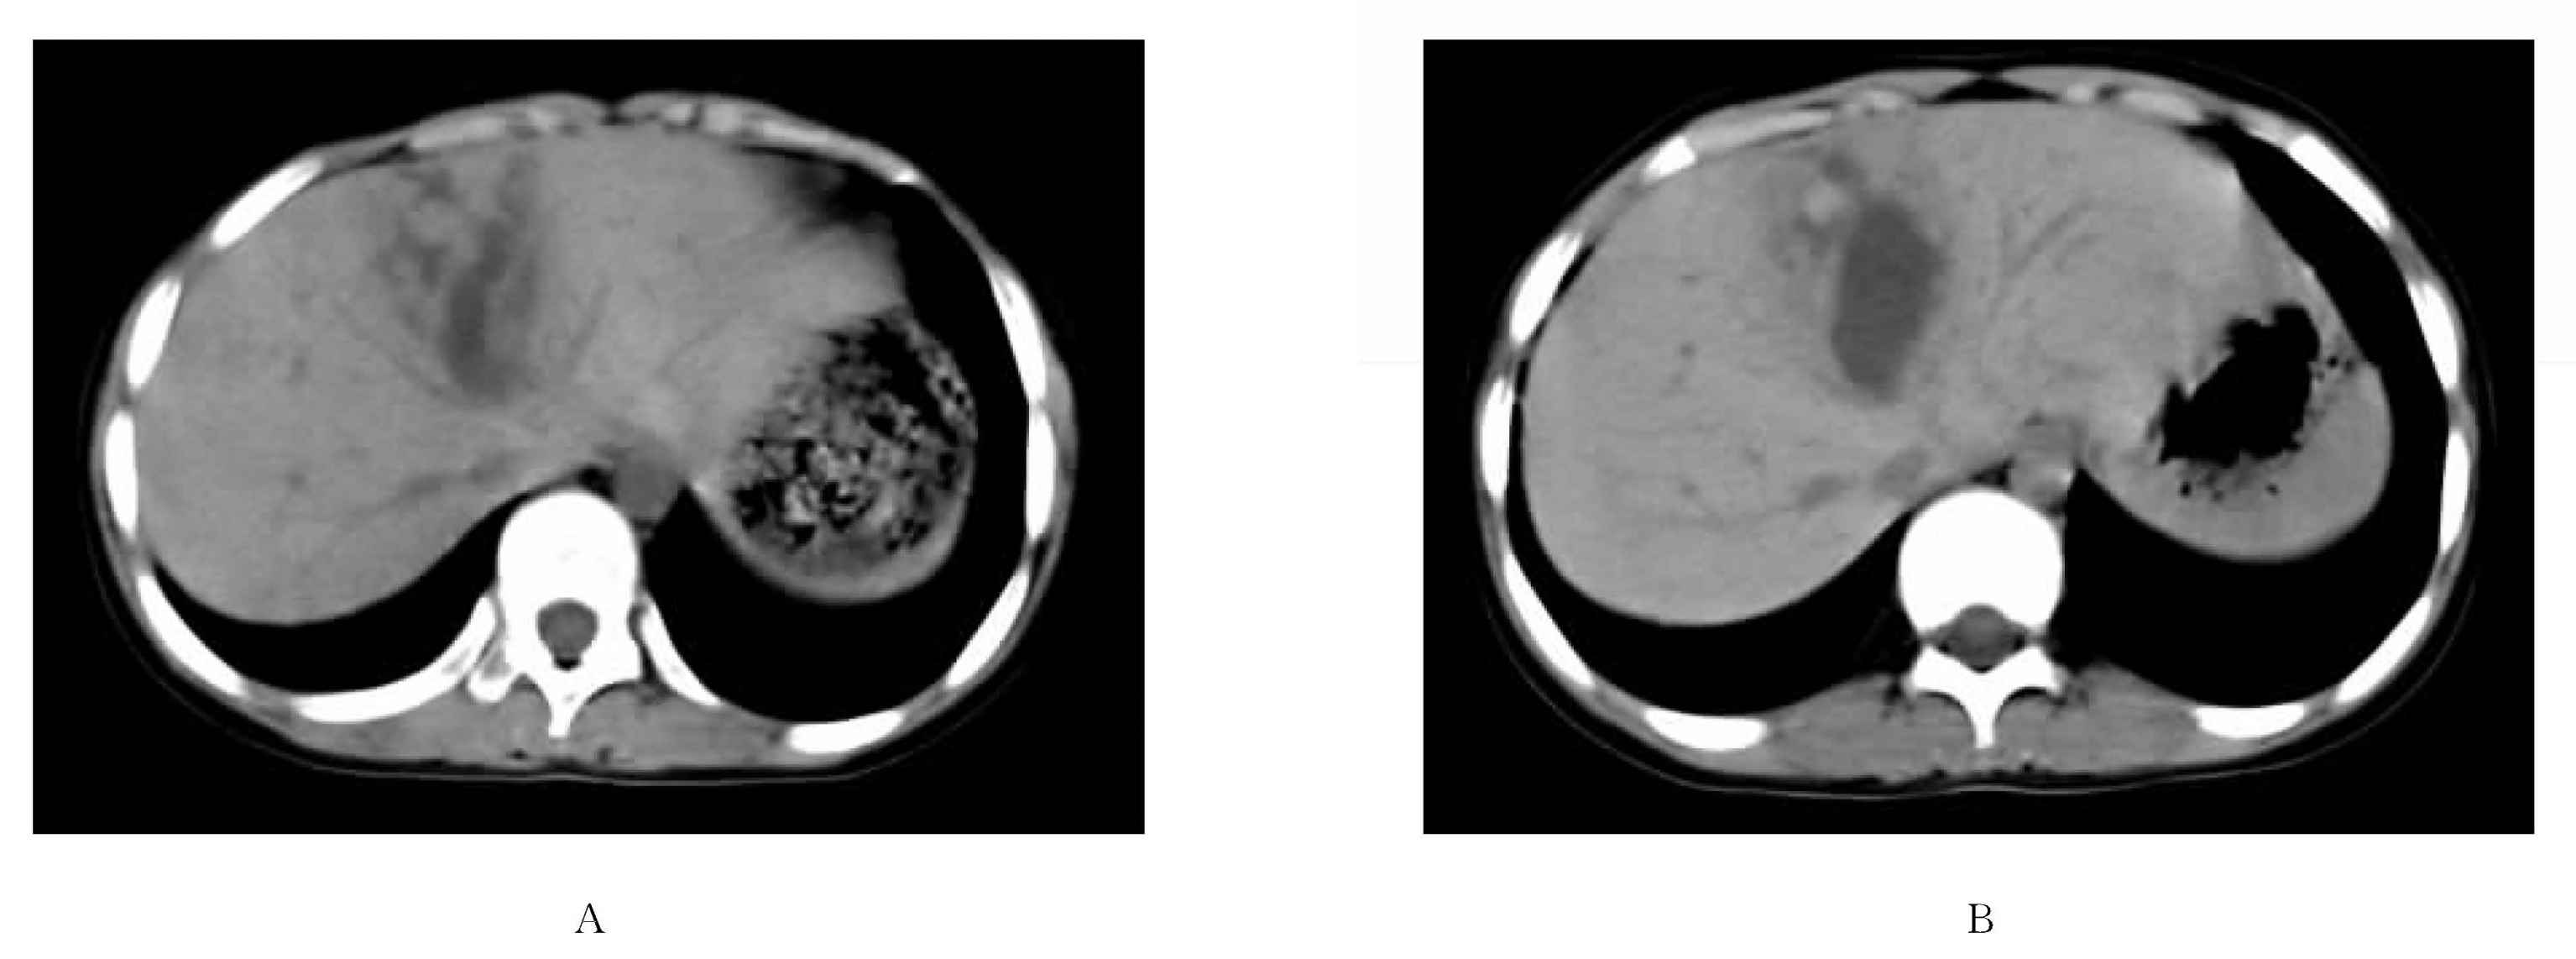
\includegraphics[width=.7\textwidth,height=\textheight,keepaspectratio]{./images/Image00392.jpg}
 \captionsetup{justification=centering}
 \caption{外伤性胆汁瘤\\{\small A为外伤后1天;B为外伤后3天,可见肝左叶内段水样低密度区逐渐增大}}
 \label{fig20-4}
  \end{figure} 

此外,腹腔积血常见。应该注意肝裸区的撕裂伤延伸至肝脏表面,可导致腹腔内积血进入腹膜后,而不形成腹膜腔积血,且体检不能发现典型的腹膜刺激征。

\textbf{【CT分级】}
肝钝性伤依据其CT表现可分为以下5级:Ⅰ级,肝包膜撕裂,表面撕裂深度<1cm,包膜下血肿大小<1cm,仅见门静脉周围轨迹征;Ⅱ级,肝撕裂深度1~3cm,肝实质和包膜下血肿大小为1~3cm;Ⅲ级,肝撕裂深度>3cm,肝实质血肿和包膜下血肿大小>3cm;Ⅳ级,肝实质血肿和包膜下血肿大小>10cm,肝组织破坏或血供中断;Ⅴ级,两叶肝组织破坏或血供中断。

\subsection{胰腺钝伤}

胰腺钝伤少见,约占腹部钝伤的5%,且常合并其他器官(如十二指肠和肝脏)的损伤。其最常见的原因为车祸。

\textbf{【病理】}
主要引起胰腺挫伤、血肿、撕裂和断裂。如果这些损伤被忽视或诊断被延误,可导致远端胰腺炎、胰腺假性囊肿形成。

\textbf{【临床表现】}
以儿童和青年更常见。主要表现为腹痛、腹部压痛以及白细胞计数增高等损伤性胰腺炎的表现。

\textbf{【CT表现】}

1.撕裂伤和断裂伤:表现为胰腺实质的中断,周围的出血位于肾旁前间隙内。

2.挫伤和血肿:可表现为胰腺弥漫性或局限性增大,或轮廓不规则。

3.其他征象:肠系膜上动脉周围的积液、横结肠系膜处的积液、胰腺与脾静脉间隙积液,以及左肾前筋膜的增厚等,但无特异性。

此外,上述征象可以延迟出现,故对疑有胰腺损伤者,如最初CT表现正常,应在12~24小时内复查。

\subsection{肾钝伤}

肾钝伤约占腹部钝伤的10%。

\textbf{【病理】}
包括肾挫伤、肾皮质撕裂伤、肾断裂伤、肾粉碎伤、包膜下血肿、创伤性肾动脉闭塞以及创伤性肾静脉栓塞。

\textbf{【临床表现】}
多有腰痛、肿胀、压痛,且多有全程肉眼血尿,少数因大量失血出现休克。

\textbf{【CT表现】} 大体有以下4方面的表现:

1.肾包膜下血肿:肾包膜下半月形、葱皮样高密度区,随时间推移而密度降低。增强扫描呈低密度,肾实质受压。

2.肾挫伤:仅表现为肾实质内边界模糊的低密度区,肾脏体积可增大。增强扫描有助于确诊。

3.肾破裂:肾实质内线样低密度裂隙,同时伴有肾周血肿(肾脂肪囊区);明显的肾周血肿常伴肾破裂。若损伤累及集合系统,可致尿液或造影剂外溢。多发严重的肾破裂可导致粉碎性肾,增强扫描有不增强的多数肾块(图\ref{fig20-5})。

\begin{figure}[!htbp]
 \centering
 
\includegraphics[width=.7\textwidth,height=\textheight,keepaspectratio]{./images/Image00393.jpg}
 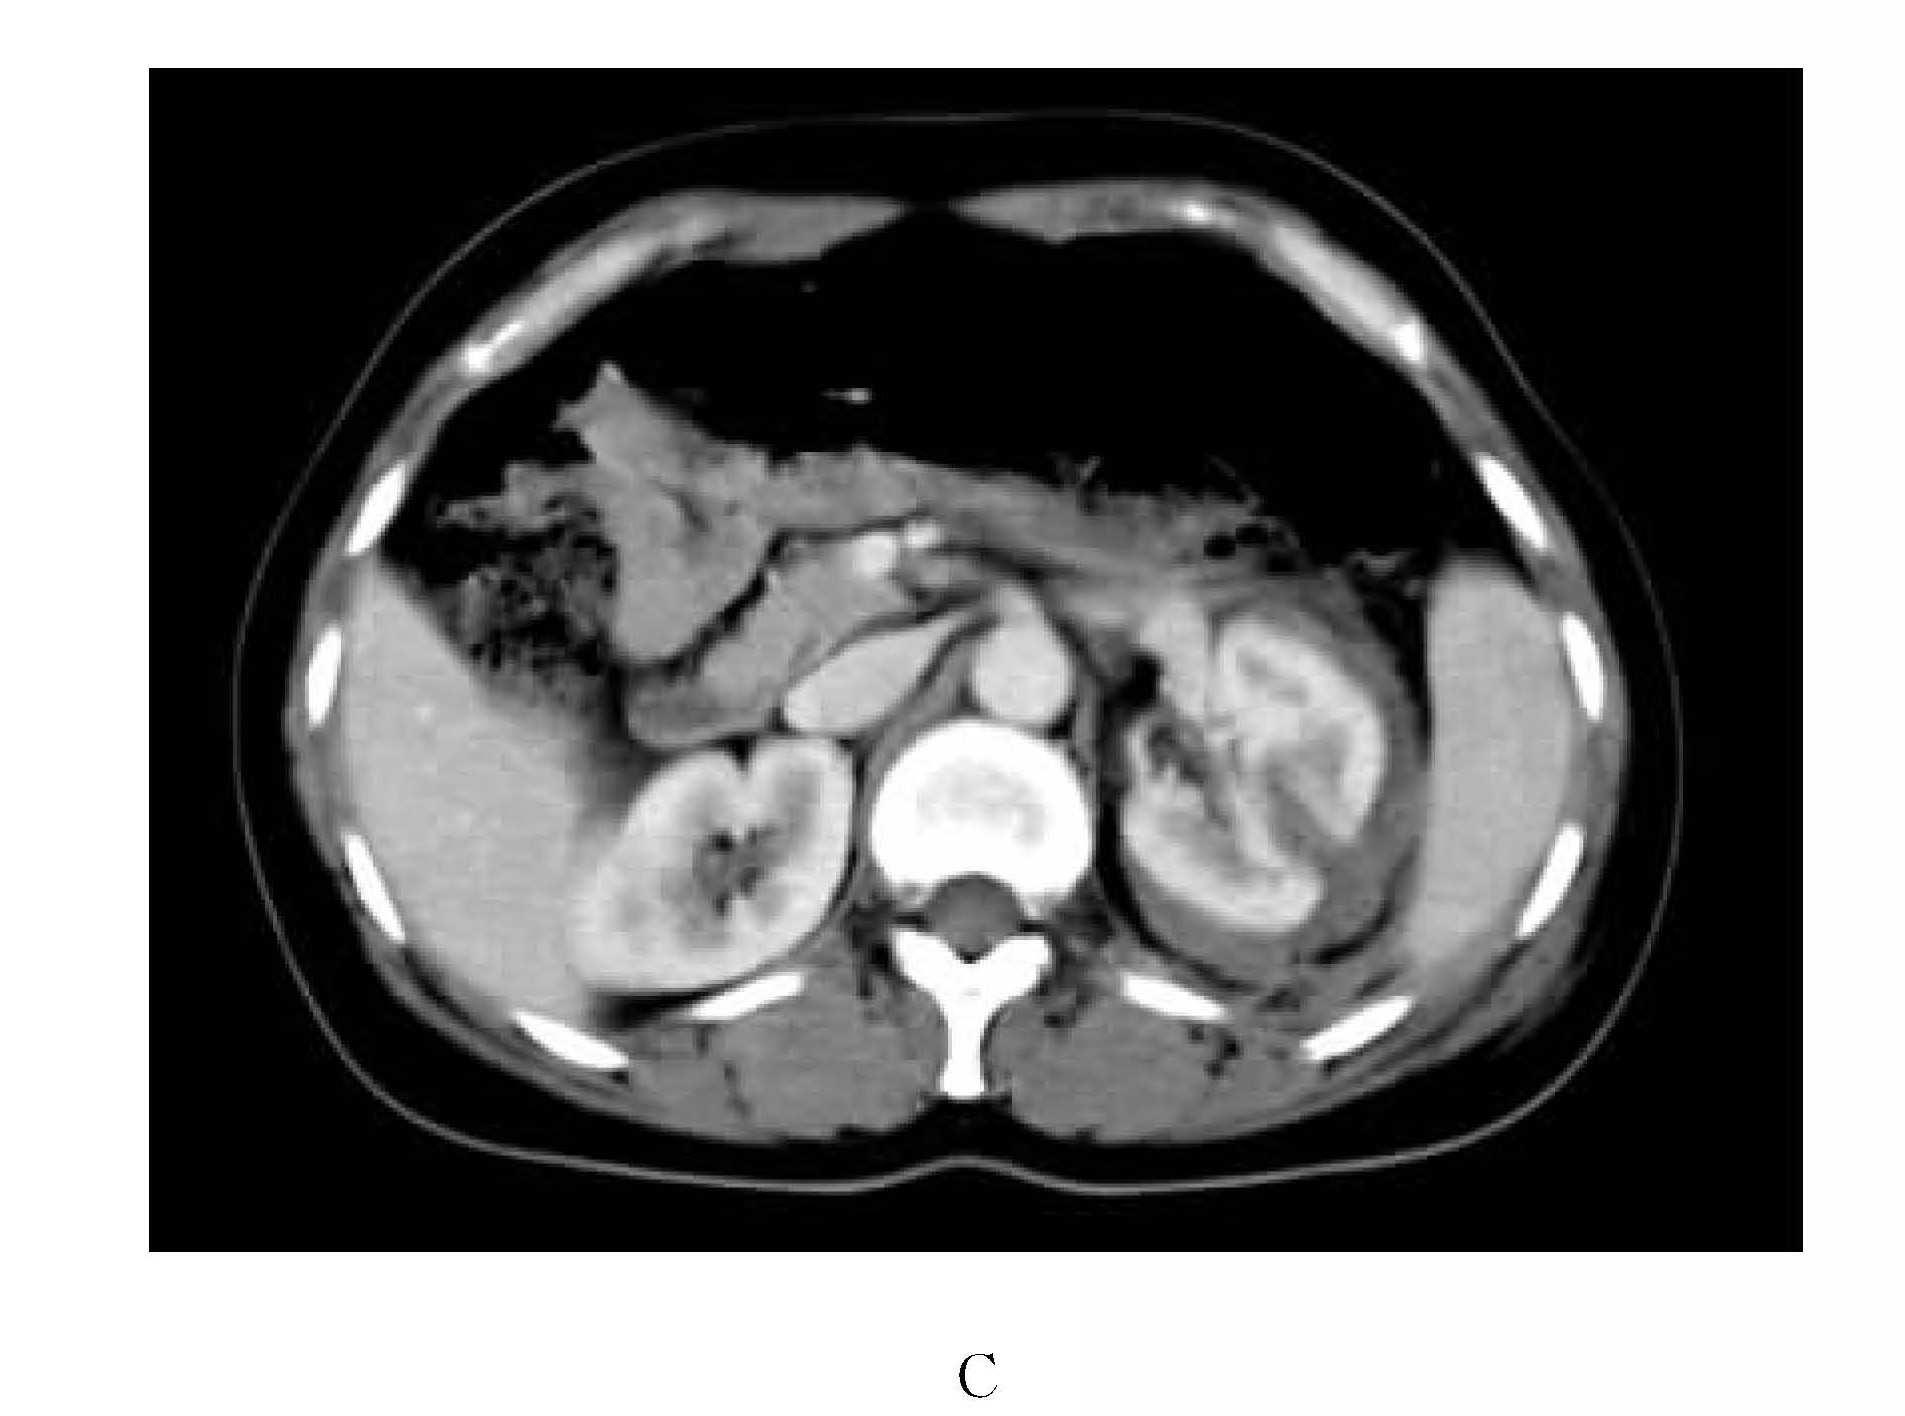
\includegraphics[width=.7\textwidth,height=\textheight,keepaspectratio]{./images/Image00394.jpg}
 \captionsetup{justification=centering}
 \caption{肾破裂\\{\small A、B为同一患者,右肾前部有高密度出血且密度不均、肾周血肿显著;增强扫描可见前部肾块不强化。C增强扫描可见左肾中部有裂隙,并可见肾周血肿}}
 \label{fig20-5}
  \end{figure} 

4.肾梗塞:①节段性肾梗塞:增强扫描呈楔形低密度区,慢性期可见薄的肾皮质增强环。②肾动脉主干闭塞:整个肾无增强,肾盂期无造影剂分泌,仅见一个薄的增强环,称为边缘征;它提示肾包膜、肾盂旁及输尿管旁存在完整的侧支动脉。

此外,国内有多个学者强调,延时5~30分钟扫描对肾损伤,尤其是收集系统损伤的诊断甚有价值。

\textbf{【CT分级】}

1.多依据美国外科创伤协会的标准分为5级。Ⅰ级,有肾挫伤或包膜下血肿,没有皮质裂伤;Ⅱ级,无扩展性的肾周血肿或裂伤<1.0cm,无尿外渗;Ⅲ级,实质裂伤延伸进入皮质>1.0cm,无尿外渗;Ⅳ级,实质裂伤超过皮髓交界处并进入集合系统;Ⅴ级,有多处重度肾破裂或有肾蒂血管伤。但上述分级应用于CT有其局限性。

2.国内有学者建议作以下分类:①肾挫伤:局部肾实质水肿,而不伴血管破裂,CT表现为局部密度减低;②肾挫裂伤:局部肾实质水肿渗出,并伴有血管破裂,CT表现为局部低密度区域内有斑点状高密度灶;③肾包膜下血肿;④肾撕裂伤;⑤肾蒂伤:肾动脉主干或分支断裂或闭塞。

\subsection{外伤性肾上腺血肿}

外伤性肾上腺血肿少见,通常胸、腹闭合伤造成肾上腺损伤的概率为1%~3%,右侧多于左侧。

\textbf{【病理机制】}
其发病与受伤部位和程度关系密切。其损伤的机制尚不明确,可能是外伤压迫下腔静脉产生的压力波,由肾上腺静脉直接传至肾上腺,肾上腺质地较脆,故易形成右肾上腺血肿。

\textbf{【临床表现】}
无典型的临床表现,可表现为右季肋部疼痛、恶心、呕吐等非特异性症状。诊断主要依赖影像学。

\textbf{【CT表现】}
血肿呈圆形或卵圆形局限或弥漫的高密度灶(图\ref{fig20-6}),边缘清晰,CT值取决于血肿的时期,增强扫描无强化或呈环状强化。约70%以上血肿边缘可见薄层肾上腺组织包绕。此外,肾上腺周围或肾上极脂肪囊内出现索条影,同侧膈肌脚可增厚。3~5个月后血肿可完全吸收,肾上腺形态恢复正常。

\begin{figure}[!htbp]
 \centering
 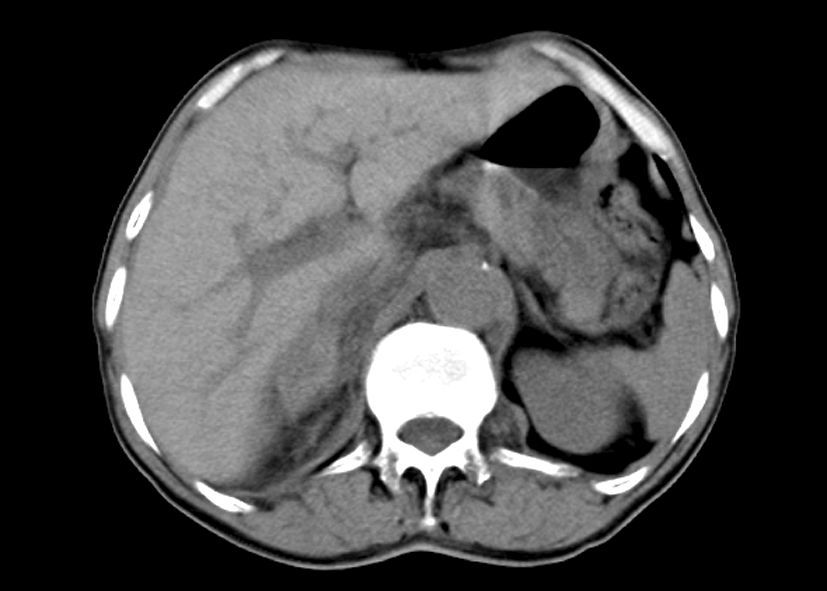
\includegraphics[width=.7\textwidth,height=\textheight,keepaspectratio]{./images/Image00395.jpg}
 \captionsetup{justification=centering}
 \caption{外伤性肾上腺血肿\\{\small 右侧肾上腺区有椭圆形稍高密度出血灶,周围有条索状高密度灶}}
 \label{fig20-6}
  \end{figure} 

\section{空腔性脏器损伤}

\subsection{肠和肠系膜损伤}

在经手术的腹部钝伤病人中,小肠和肠系膜损伤者占50%,亦可为贯通性损伤。

\textbf{【临床表现】}
腹痛、腹胀和弥漫性腹膜刺激征,严重者可有出血性休克。

\textbf{【CT表现】}
①气腹;②口服造影剂外溢;③腹膜腔和腹膜后腔积液;④肠壁增厚;⑤受累肠区附近出现高密度血块和局部肠系膜出血或血肿(图\ref{fig20-7})。

\begin{figure}[!htbp]
 \centering
 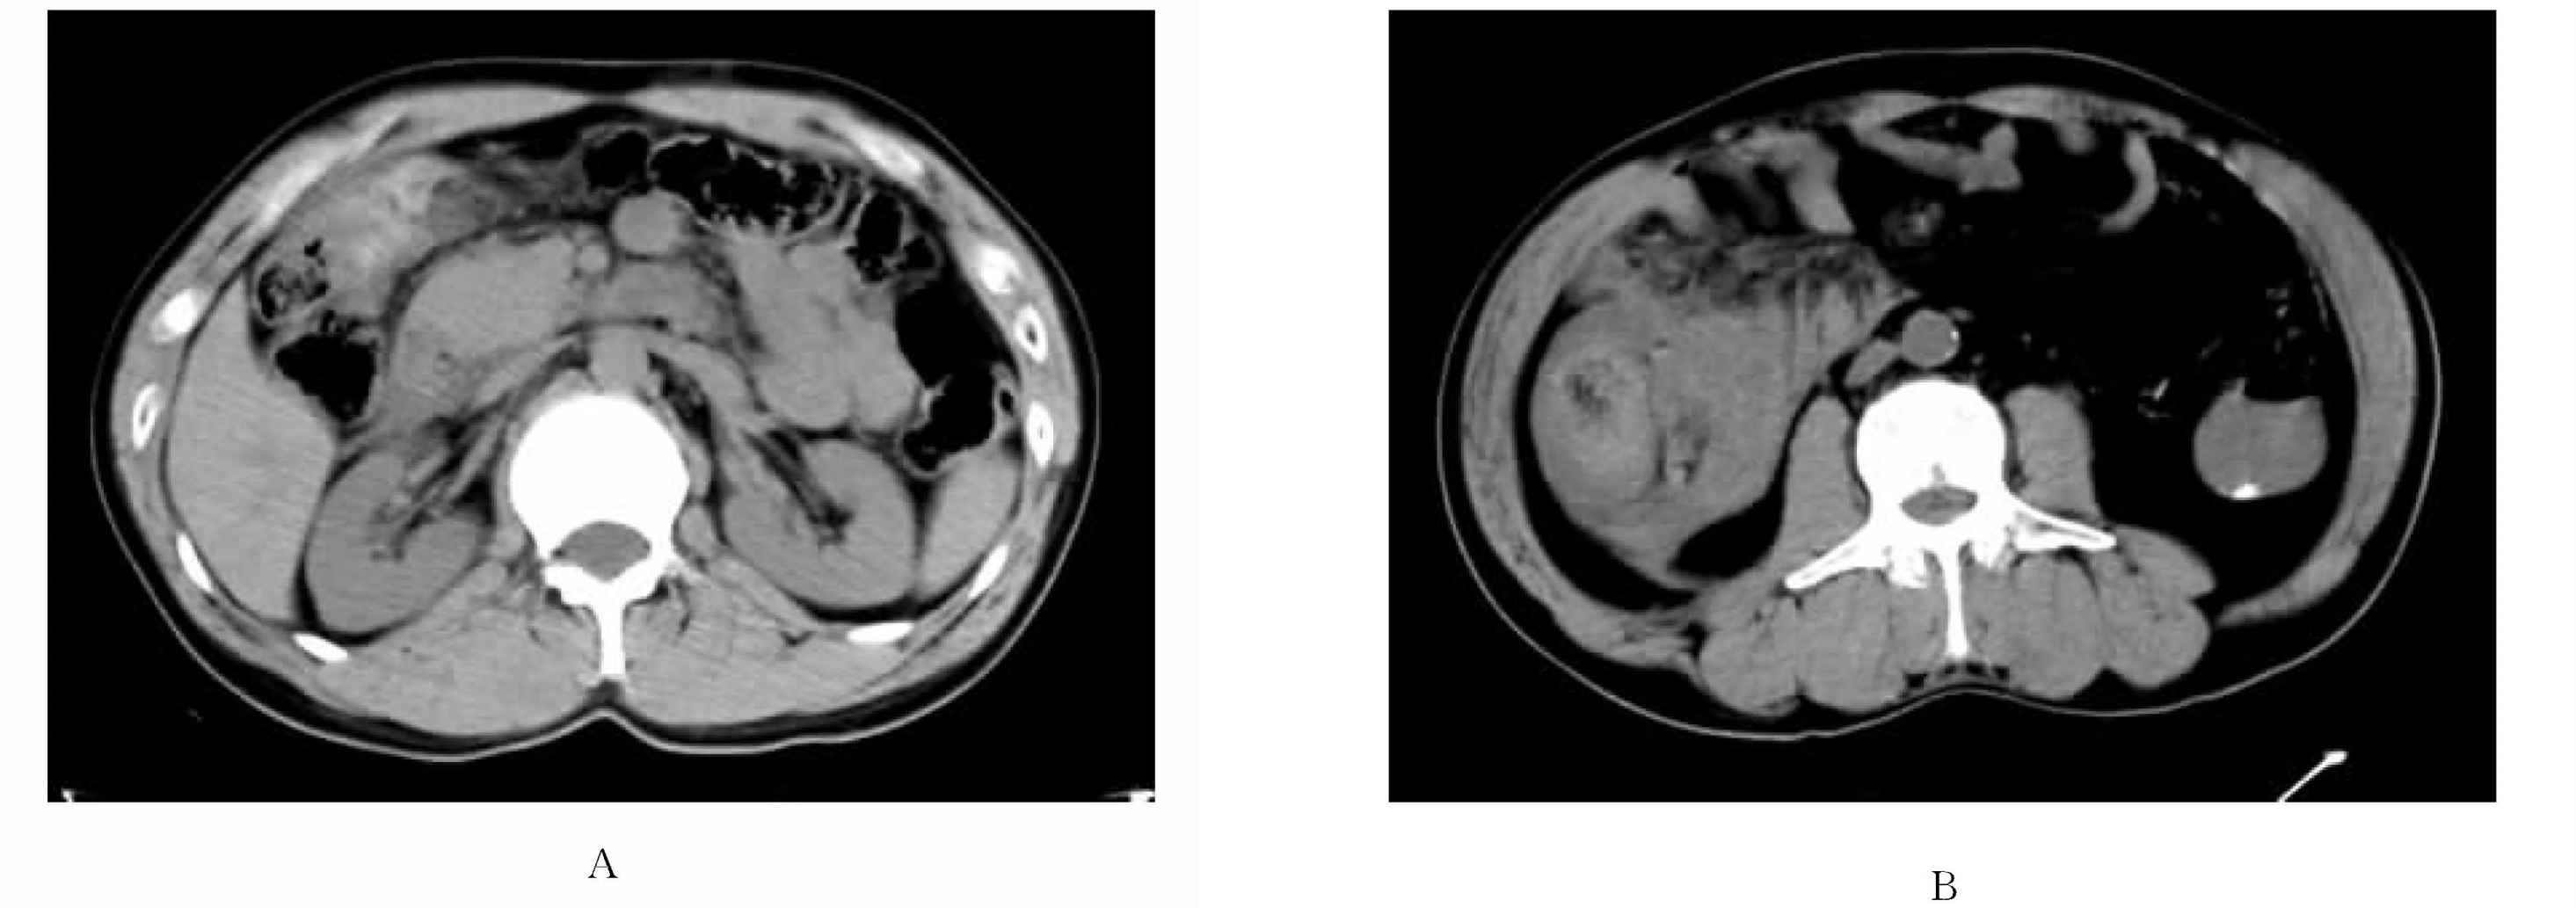
\includegraphics[width=.7\textwidth,height=\textheight,keepaspectratio]{./images/Image00396.jpg}
 \captionsetup{justification=centering}
 \caption{肠系膜出血\\{\small A、B非同一患者,在腹腔右侧均有局限性稍高密度的出血区,密度不均匀}}
 \label{fig20-7}
  \end{figure} 

腹腔中量或大量积液,如没有发现实质性器官损伤应怀疑肠或肠系膜损伤。局限性肠系膜浸润亦常见,但无特异性。约75%的肠壁撕裂能看到肠壁增厚。肠系膜增厚常提示胃肠穿孔。此外,腹腔积气可由纵隔积气、气胸或诊断性腹腔穿刺所致,应注意鉴别。

\subsection{腹腔间隙综合征}

该征在严重创伤及其他危重病患者中具有较高的发病率。

\textbf{【病理机制】}
其机制尚未完全阐明。目前认为主要与血管渗漏、缺血再灌注损伤、血管活性物质释放以及氧自由基等综合作用导致脏器水肿、细胞外液大量增加有关。特别是在严重创伤后需要快速大量输液复苏的患者,由于血管通透性增加、内脏器官水肿和腹水使脏器容积增加,引起腹内高压而导致该征的发生。

\textbf{【CT表现】}
国外有学者提出其CT诊断征象是:下腔静脉狭窄、肾脏受压或移位、肠壁增厚和圆腹征表现。国内学者则归纳为:①腹腔大量积液、腹内高压并圆腹征;②肠壁增厚征;③腹腔脏器间间隙闭合征;④肠系膜广泛肿胀模糊征;⑤小肠黏膜“羽毛征”、“弹簧征”和“齿轮征”;⑥胰腺肿胀增粗征;⑦肾脏受压或移位、肾动静脉及下腔静脉狭窄征;⑧双侧胸腔积液征。

\subsection{胆囊创伤}

胆囊创伤罕见。钝性创伤常发生在胆囊充满胆汁或扩张时,常合并肝脏和十二指肠的损伤。

\textbf{【病理】} 其损伤包括胆囊壁的挫裂伤、胆囊破裂和胆囊撕脱。

\textbf{【CT表现】}
胆囊是腹膜间位器官,胆汁从破裂的胆囊可渗到胆囊窝内,但渗到腹膜腔的征象少见。主要征象有:①胆囊周围积液(最常见);②胆囊轮廓毛糙;③胆囊壁局限性增厚或不连续;④胆囊腔内出血。此外,胆囊撕脱可见胆囊动脉及其分支的破裂处明显出血。

\subsection{膀胱损伤}

膀胱损伤并不常见,但10%~15%伴有严重的骨盆骨折。

\textbf{【病理】} 其损伤包括膀胱挫伤和膀胱破裂。

\textbf{【CT表现】}
①挫伤:表现为壁内血肿和膀胱壁增厚。②破裂:可以发生于腹膜腔内或腹膜腔外。平扫表现为膀胱内高密度出血在下层,低密度尿液在上层。如膀胱内无尿液充盈,则膀胱壁及膀胱内分布多个大小不等的片状出血,膀胱形态不完整。增强扫描可显示破裂的膀胱壁和外溢的造影剂。

\textbf{【鉴别诊断】}
膀胱破裂应与膀胱憩室相鉴别。后者有光滑的颈部,膀胱壁完整,无造影剂外溢。

\protect\hypertarget{text00028.html}{}{}

